\documentclass[11pt]{article}

\usepackage[utf8]{inputenc}
\usepackage[T1]{fontenc}
\usepackage{lmodern}
\usepackage[margin=1in]{geometry}
\usepackage{setspace}
\usepackage{microtype}
\usepackage{amsmath,amssymb,amsthm,mathtools}
\usepackage{booktabs,longtable}
\usepackage{graphicx}
\usepackage{float}
\usepackage[section]{placeins}
\usepackage{xurl}
\usepackage[colorlinks=true,linkcolor=blue,urlcolor=blue]{hyperref}

\onehalfspacing
\graphicspath{{figures/}}
\emergencystretch=2em
\renewcommand{\thesection}{S\arabic{section}}
\renewcommand{\thefigure}{S\arabic{figure}}
\renewcommand{\thetable}{S\arabic{table}}
\renewcommand{\theequation}{S\arabic{equation}}

\newcommand{\Pbb}{\mathbb{P}}
\newcommand{\Ebb}{\mathbb{E}}
\newcommand{\Fcal}{\mathcal{F}}
\newcommand{\Mcal}{\mathcal{M}}
\newcommand{\Acal}{\mathcal{A}}
\newcommand{\Hcal}{\mathsf{H}}
\newcommand{\norm}[1]{\left\lVert #1\right\rVert}

\title{Supporting Information for\\
Extra Hidden States under Emission Misspecification in Hidden Markov Models}
\author{Aur\'elien Nicosia\\
D\'epartement de math\'ematiques et de statistique, Universit\'e Laval}
\date{}

\begin{document}
\maketitle

\section{Proofs}\label{sec:proofs}

This section gives the proofs of Lemma~2.3, Propositions~2.4--2.5,
Theorem~2.6, and Corollary~2.7 from Section~2 of the main article, in that
order. Notation is identical to that article. For convenience, the
Kullback--Leibler divergence and $L^1(\lambda)$ distance used below are
$D(p\Vert q)=\int p\log(p/q)\,d\lambda$ and
$\norm{p-q}_1=\int|p-q|\,d\lambda$, with the extended-value conventions stated
in the main article. Also let
$\Delta_K=\{(\omega_1,\ldots,\omega_K)\in[0,1]^K:
\sum_{j=1}^K\omega_j=1\}$ denote the $K$-weight probability simplex.

\subsection{Proof of Lemma~2.3: separation from lower-order mixtures}

The class $\Mcal_{K_0}$ is the continuous image of the compact set
$\Delta_{K_0}\times\Theta^{K_0}$ and is therefore compact in $L^1$. The
constrained simplex defining $\Acal_c$ is compact, so $\Acal_c$ is compact as
well. The sets are disjoint. Otherwise, a mixture containing exactly $R$
positive-weight, pairwise distinct atoms would equal a mixture with at most
$K_0$ atoms after zero-weight and repeated atoms were removed. This contradicts
identifiable minimal order. Two disjoint compact sets in a metric space have
positive distance, hence
\begin{equation*}
 d_c=\inf_{p\in\Acal_c}\inf_{q\in\Mcal_{K_0}}\norm{p-q}_1>0.
\end{equation*}
Pinsker's inequality, $D(p\Vert q)\geq\norm{p-q}_1^2/2$, then gives the claimed
Kullback--Leibler lower bound.

\subsection{Proof of Proposition~2.4: aligned improvement by state splitting}

In the aligned comparison, the hidden aggregate trajectory law is held fixed.
All transition terms therefore cancel in the complete-data likelihood ratio.
With one fitted emission $f_{\eta_k}$ per state, stationarity gives the risk
\begin{equation*}
 \mathcal{R}(f_{\eta_1},\ldots,f_{\eta_{K_0}})=\sum_{k=1}^{K_0}\pi_k\,D(g_k\Vert f_{\eta_k}).
\end{equation*}
Taking the infimum over the emission parameters gives
$\sum_k\pi_k\delta_k(1)$. With $m_k$ substates, the fitted aggregate emission
can be any $q_k\in\Mcal_{m_k}$ by drawing a component independently
at each visit to state $k$, as in the refinement construction, yielding
$\sum_k\pi_k\delta_k(m_k)$. Since
$\Mcal_1\subseteq\Mcal_{m_k}$, all terms weakly decrease. A strict decrease in
one state with $\pi_k>0$ proves the strict inequality when the original
weighted risk is finite. Without that condition another state can have
infinite loss under both models, leaving both total risks infinite; only
the non-increase is then guaranteed.

\subsection{Proof of Proposition~2.5: exact HMM refinement}

Let $X_t^{\mathrm{ref}}$ denote the refined chain and let $r(k,a)=k$ map a
refined state to its aggregate state. The refined transition matrix is
stochastic because
\begin{equation*}
 \sum_{\ell,b}\gamma^0_{k\ell}\omega^0_{\ell,b}=1.
\end{equation*}
The distribution $\pi_k\omega^0_{k,a}$ is stationary since
\begin{equation*}
 \sum_{k,a}\pi_k\omega^0_{k,a}\gamma^0_{k\ell}\omega^0_{\ell,b}
 =\omega^0_{\ell,b}\sum_k\pi_k\gamma^0_{k\ell}
 =\pi_\ell\omega^0_{\ell,b}.
\end{equation*}
Furthermore,
\begin{equation*}
 \Pbb\{r(X_t^{\mathrm{ref}})=\ell\mid X_{t-1}^{\mathrm{ref}}=(k,a)\}
 =\sum_b\gamma^0_{k\ell}\omega^0_{\ell,b}=\gamma^0_{k\ell}.
\end{equation*}
Summing the refined joint density over substate paths compatible with a fixed
aggregate path $z_{1:T}=(z_1,\ldots,z_T)$ gives
\begin{align*}
 &\pi_{z_1}\prod_{t=2}^T\gamma^0_{z_{t-1},z_t}
 \prod_{t=1}^T\sum_{a=1}^{m_{z_t}}
 \omega^0_{z_t,a}f_{\eta^0_{z_t,a}}(y_t)\\
 &\qquad=\pi_{z_1}\prod_{t=2}^T\gamma^0_{z_{t-1},z_t}
 \prod_{t=1}^T g_{z_t}(y_t).
\end{align*}
Summing over aggregate paths proves equality of all observed
finite-dimensional distributions.

\subsection{Proof of Theorem~2.6: observed-law separation}

Exact refinement establishes
\begin{equation*}
 \inf_{Q\in\Hcal_R(\Fcal)}
 \underline D^{\mathrm{rate}}(P_0^Y\Vert Q)=0.
\end{equation*}

Write $\Pbb_0$ and $\Ebb_0$ for probability and expectation under the true
aggregate HMM\@. Fix a candidate $Q\in\Hcal_{K_0}(\Fcal)$ with emissions
$f_{\eta_1},\ldots,f_{\eta_{K_0}}$. Let
$\beta^Q_{t,j}(y_{1:t-1})$ be its predictive probability of hidden state $j$
given the realized observation history
$y_{1:t-1}=(y_1,\ldots,y_{t-1})$. Its one-step predictive density has the form
\begin{equation*}
 p_t^Q(y\mid y_{1:t-1})
 =\sum_{j=1}^{K_0}\beta^Q_{t,j}(y_{1:t-1})f_{\eta_j}(y),
\end{equation*}
where the $\beta^Q_{t,j}$ are nonnegative and sum to one. Thus the predictive
density belongs to $\Mcal_{K_0}$ for every history, regardless of the candidate
transition matrix and initial distribution.

For the true aggregate HMM, let
\begin{equation*}
 \beta^0_{t,k}(y_{1:t-1})
 =\Pbb_0(Z_t=k\mid Y_{1:t-1}=y_{1:t-1}).
\end{equation*}
Stationarity implies
$\pi_\ell=\sum_k\pi_k\gamma^0_{k\ell}\geq\varepsilon$, so
$\beta^0_{1,\ell}\geq\varepsilon$. For $t\geq2$,
\begin{align*}
 \beta^0_{t,\ell}(y_{1:t-1})
 &=\sum_k\Pbb_0(Z_{t-1}=k\mid Y_{1:t-1}=y_{1:t-1})
 \gamma^0_{k\ell}\\
 &\geq\varepsilon.
\end{align*}
The true predictive density is consequently
\begin{equation*}
 p_t^0(y\mid Y_{1:t-1})
 =\sum_{k,a}\beta^0_{t,k}(Y_{1:t-1})\omega^0_{k,a}
 f_{\eta^0_{k,a}}(y),
\end{equation*}
with every refined weight at least $c=\varepsilon\omega_{\min}$. Thus
$p_t^0(\cdot\mid Y_{1:t-1})\in\Acal_c$ almost surely. By the
mixture-separation lemma,
\begin{equation*}
 D\{p_t^0(\cdot\mid Y_{1:t-1})\Vert
 p_t^Q(\cdot\mid Y_{1:t-1})\}\geq d_c^2/2
\end{equation*}
almost surely. If a conditional divergence is infinite, the desired bound is
immediate. Otherwise, the chain rule gives
\begin{align*}
 D\{(P_0^Y)^{1:T}\Vert Q^{1:T}\}
 &=\sum_{t=1}^T\Ebb_0\left[
 D\{p_t^0(\cdot\mid Y_{1:t-1})\Vert
 p_t^Q(\cdot\mid Y_{1:t-1})\}\right]\\
 &\geq Td_c^2/2.
\end{align*}
This proves the finite-sequence assertion for every $T\geq1$.
Dividing by $T$ and taking a lower limit proves the positive
relative-entropy-rate bound.

\subsection{Proof of Corollary~2.7: enriched-emission representation}

Each true emission $g_k$ belongs to $\Mcal_M$ when
$M\geq\max_{1\leq k\leq K_0}m_k$. The original aggregate chain is therefore an
element of
$\Hcal_{K_0}(\Mcal_M)$ with observed law $P_0^Y$, and the infimum of the
relative-entropy rate is zero.

\section{Simulation computation and diagnostics}\label{sec:simulation-si}

The accompanying reproducibility files contain the simulation, genomic and
supplementary movement analyses. The simulation repository is
\url{https://github.com/AurelienNicosiaULaval/corrective-hmm-states}.
The replicated study is regenerated from the package root with
\path{numerics/scripts/run_optimization_audit.R}, using master seed
\texttt{20260610}. The compiled EM implementation is checked against the
public R updates for four component specifications, both single and multiple
sequences, and three iteration counts.

The study compares Gaussian HMMs with two and three states and a two-state
HMM with two Gaussian components per state. There are 200 fixed-seed
replications at each of $T\in\{500,1500,5000\}$. Ten random starts use the
same initial distributions as the original protocol, with 25 screening
iterations for Gaussian models and 30 for mixtures, followed by refinement
of the best three. Additional starts are constructed from fitted data:
splitting a G2 emission or reducing an M22 emission supplies a candidate
M21 model; exact M21 refinement supplies a G3 start, and duplicating its
single component supplies an M22 start. The generating parameters are
never used as initial values. Refinement uses relative log-likelihood
tolerance $10^{-9}$ in blocks of up to 3,000 iterations, continued until
convergence. The standard-deviation floor is 0.05.

The final G3 and M22 likelihoods must be at least the fitted M21 likelihood,
and all three reported fits must improve or retain their original
likelihoods. The per-replication parameters, stopping diagnostics, original
results and comparisons are retained in
\path{numerics/output/optimization_audit}. These checks address observed
optimization failures without proving global optimality.
The R and compiled implementations add $10^{-10}$ to initial-state and
transition counts, and $10^{-12}$ to active component counts and emission
update denominators. These numerical safeguards do not change the stated
model classes.

Model comparisons use the Bayesian information criterion (BIC), as defined in
the main article. Row-level results are stored in
\path{numerics/output/review_replications.csv}; the compact summary is in
\path{numerics/output/review_summary_by_T.csv}. Additional diagnostics appear
in Figures~\ref{fig:si-posterior}--\ref{fig:si-acf}.

\begin{figure}[p]
\centering

\includegraphics[width=.82\linewidth]{posterior_corrective_state.pdf}
\caption{Posterior probability of the corrective Gaussian-HMM state in the
reference $K=3$ fit. The probability tracks observations associated with the
second component of the heterogeneous first aggregate regime.}
\label{fig:si-posterior}
\end{figure}

\begin{figure}[p]
\centering

\includegraphics[width=.82\linewidth]{bic_boxplot.pdf}
\caption{Distribution of the BIC difference between the three-state and
two-state Gaussian models over the $T=1500$ replications. Negative values
favour the corrective three-state Gaussian HMM.}
\label{fig:si-bic-boxplot}
\end{figure}

\begin{figure}[p]
\centering

\includegraphics[width=.82\linewidth]{residual_acf.pdf}
\caption{Autocorrelation of approximate one-step standardized prediction
residuals for the Gaussian-emission HMMs with $K=2$ and $K=3$.}
\label{fig:si-acf}
\end{figure}

\section{Genomic application details}\label{sec:genomic-si}

\subsection{Provenance, preprocessing and partition}

The original Affymetrix SNP 6.0 CEL files are from Gene Expression Omnibus
(GEO), series \href{https://www.ncbi.nlm.nih.gov/geo/query/acc.cgi?acc=GSE13372}{GSE13372},
associated with Chiang et al. (2009),
\url{https://doi.org/10.1038/nmeth.1276}.
The first pair comprises GSM337641 (HCC1143) and GSM337662 (HCC1143BL);
the second comprises GSM337642 and GSM337663. Their selection follows
accession order, rather than a comparison of fitted profiles. Their download locations and SHA-256 hashes are recorded in the source
manifest.
These arrays are repeated measurements of the same cell line and matched
normal, not four independent biological specimens.

AS-CRMAv2 in aroma.affymetrix 3.2.3 processes each array; the exported total
signals and B fractions contain 1,881,415 assay units. TumorBoost v4 in
aroma.light 3.38.0 corrects tumor fractions using the matched normal, with
heterozygous normal target $\mu_N=0.5$ and \texttt{preserveScale=FALSE}.
The procedure and correction are described by Bengtsson et al. (2009, 2010),
\url{https://doi.org/10.1093/bioinformatics/btp371} and
\url{https://doi.org/10.1186/1471-2105-11-245}.
The matched normal serves two roles: it identifies candidate heterozygous
markers, at which both A and B variants are present, and supplies the
reference for marker-specific fraction correction. One observation in the
HMM is the resulting corrected tumor fraction at a retained genomic position.
Corrected values outside $[0,1]$ are possible and are retained. Gaussian
measurement densities are fitted to these corrected fractions, not to
bounded counts or latent allele probabilities.

Analysis coordinates come from
\path{GenomeWideSNP_6,Full,na30,hg18,HB20100215.ugp}.
The hg19 annotation used by the preprocessing environment for other purposes
is not used to align the published sequencing boundaries. We require finite
fractions, positive positions and matched-normal fractions in $[0.3,0.7]$.
At duplicate chromosome/position pairs, the first assay-unit index is retained.
Chromosome 1 initially has 146,401 assay units, of which 73,346 have finite
paired fraction measurements and 20,786 pass the normal-fraction filter;
20,697 unique-position markers remain. The two sequences contain 10,322 and
10,375 markers. Consecutive retained positions more than one megabase apart
start a new sequence, as does every chromosome change.

The local protocol was recorded before inspecting processed profiles or
fitting HMMs. Chromosome 1 was designated for initial development;
chromosomes 2--11 were reserved as possible extensions but were unused.
Chromosomes 12--17 were validation, and 18--22 were not evaluated until the
fitted model files and specification had been hashed and frozen. This is a
local exploratory design, not an externally registered confirmatory study.
The saved model objects and written protocol match the recorded freeze
hashes; the distributed evaluation script is a later version. Here
``confirmation'' denotes a later held-out block within this exploratory
analysis, rather than preregistered confirmatory inference.
No chromosome outside chromosome 1 contributes to parameter estimation.
The second array pair assesses technical repeatability on chromosome 1.

\subsection{Estimation and numerical checks}

All ordinary and unconstrained mixture models use the EM updates in the
main article. The likelihood is a product over explicitly reset sequences;
initial-state updates average responsibilities at all sequence starts, and
transition updates exclude sequence boundaries. The standard-deviation floor
is 0.01 on the corrected-fraction scale. The ordinary and unconstrained
mixture implementations use the numerical pseudocounts stated in SI S2.
Forty random starts receive up to
100 screening iterations at relative tolerance $10^{-5}$, followed by up to
2,500 iterations at $10^{-8}$ for the best eight. Persistent initializations
use diagonal transition probabilities 0.95, 0.995 and 0.9995. For G2 these
include a common centre of 0.5 with different variances: allowing only
separated-mean starts missed the higher-likelihood variance-regime fit.
Mixture starts supplement random initializations with low/high pairs.
Selections are always based on likelihood, not on appealing decoded labels.

G2 is included in M21 by duplicating an emission component. M21 is included
in G3 by the exact refinement; G3 is included in M221 by duplicating the
first two component distributions. A duplicated aggregate state additionally
embeds M21 in M221. Finally, M221 is included in G5 by exact refinement.
The code checks the likelihood at these inclusions and refines from them,
including small separation perturbations. The selected G3 and G5 likelihoods
must be at least those of M21 and M221. The tests independently compare the
multiple-sequence recursion with direct path enumeration and verify that
changing later observations cannot alter earlier predictive probabilities.

\begin{table}[htbp]
\centering
\small
\caption{Selected estimates on chromosome 1. Runs count consecutive Viterbi labels within each sequence; they are not verified genomic alterations.}
\label{tab:si-genomic-estimation}
\begin{tabular}{lrrrr}
\toprule
Model & $\ell$ & Runs & Converged & Floor hits \\
\midrule
G2 & 7410.531 & 14 & TRUE & 0 \\
M21 & 10436.225 & 78 & TRUE & 0 \\
G3 & 10438.681 & 4009 & TRUE & 0 \\
M221 & 12508.295 & 181 & TRUE & 0 \\
G5 & 12517.423 & 9123 & TRUE & 0 \\
F2 & 10980.247 & 68 & TRUE & 0 \\
F3 & 12487.146 & 184 & TRUE & 0 \\
\bottomrule
\end{tabular}
\end{table}


The unrestricted five-state model has a minimum transition estimate of about
$1.29\times10^{-7}$. This is not a zero transition or proof of structural
absence. The lower variance bound is inactive in every selected primary fit.
Relative convergence of EM and multiple starts do not prove global optimality;
all screened and refined likelihoods are retained in the fitted objects.

For F2 and F3, the E-step uses the two reflected normal contributions within
each state. The M-step ties their variances, weights them equally and updates
a nonnegative separation from one half. Thirty starts receive 120 screening
iterations; the best six are refined for up to 3,000 iterations at tolerance
$10^{-8}$. Initial and transition probabilities have a $10^{-6}$ lower bound.
Scores are densities of the original signed fraction, so no folded-density
factor is inadvertently added to comparisons with G2--G5 or M21/M221.
Direct enumeration, likelihood ascent and exact invariance under independent
allele flips are tested. F3's fitted separations are 0.0041, 0.1048 and 0.3101.
The nearly zero first separation is another reason not to use regular
asymptotic mixture-order tests.

\paragraph{Likelihood-ratio calibration for the refinement constraints.}
The prespecified grouping has two paired emissions and one single emission.
The likelihood ratio compares M221 with its unrestricted five-state Gaussian
refinement, including the corresponding initial-distribution constraints.
The statistic after numerical refinement is 18.2582; the saved primary fits
give 18.2572, a difference of approximately 0.001. The refined null and
alternative log likelihoods improve by less than 0.001 each and leave the
reported comparison unchanged at its stated precision.

The parametric bootstrap uses 199 independent simulations from the refined
M221 fit, with sequence lengths 10,322 and 10,375. Each sequence starts from
the common fitted initial distribution. Simulation seeds are
$202609170+b$, $b=1,\ldots,199$, with fitting seeds offset by 10,000.
For both observed and simulated data, each model screens ten random starts
and starts at the saved primary parameters for 100 iterations. These saved
parameters come from the observed data: they provide preoptimized starts for
the observed series but serve as warm starts for each simulated series.
The best four
are refined at relative likelihood tolerance $10^{-8}$; the alternative also
retains and refines the exact expansion of its fitted null. All selected
fits satisfy the stopping criterion and all alternative likelihoods are at
least their null likelihoods. Parameters, traces and seeds are saved in
\path{genomics/results/refinement_bootstrap}; the executable script is
\path{genomics/scripts/genomic_refinement_bootstrap.R}.

Seventeen simulated statistics meet or exceed the observed value. The
plus-one estimate is 0.09, with Monte Carlo standard error 0.020; the exact
95\% binomial interval for the underlying bootstrap tail probability is
$[0.051,0.133]$. This interval describes Monte Carlo uncertainty only.
For comparison, the bootstrap mean and 95\% quantile are 12.3 and 21.1;
the corresponding $\chi^2_{12}$ values are 12 and 21.0, and its tail
probability at 18.2582 is 0.108. Agreement of these summaries is descriptive;
it does not establish the assumptions of the asymptotic reference law.
The bootstrap is conditional on M221 being an adequate observation model;
it does not correct residual dependence or validate a biological partition.
Because the initial distribution is estimated from two sequence starts,
we do not use the difference of 14 free parameters as automatic chi-squared
degrees of freedom. The stationary-law result of Holzmann and Schwaiger
(2015), discussed in the main article, concerns different initial-law
assumptions. We report the bootstrap as an approximate calibration of this
specified constrained comparison, not as a new state-reduction test.

\subsection{Prediction and calibration}

Sequential held-out log scores use the previous forward filter and fixed
training parameters. Each validation or confirmation sequence starts with
the fitted initial distribution, not a state estimated from the full held-out
path. Smoothed states are used only for descriptive assignment and are never
substituted into the predictive density. Table~\ref{tab:si-genomic-chromosomes}
gives all chromosome-specific differences. F3's predictive advantage on some
chromosomes is retained; the analysis does not select a comparator on the
basis of which one makes M221 look best.

\begin{table}[htbp]
\centering
\small
\caption{Predictive log-score differences with parameters fixed at the development fit. Positive values favour M221. Chromosomes 12--17 are validation; chromosomes 18--22 are confirmation.}
\label{tab:si-genomic-chromosomes}
\begin{tabular}{lrrr}
\toprule
Chromosome & $n$ & M221 $-$ G5 & M221 $-$ F3 \\
\midrule
12 & 12637 & 10.076 & 10.329 \\
13 & 9646 & 1.514 & 4.708 \\
14 & 8395 & 3.741 & -0.043 \\
15 & 7493 & 12.151 & -1.256 \\
16 & 8071 & 6.123 & -6.185 \\
17 & 6052 & 2.644 & -0.555 \\
18 & 7766 & 1.190 & -4.056 \\
19 & 3823 & -0.776 & 0.212 \\
20 & 6482 & -5.826 & -14.973 \\
21 & 3767 & 10.934 & 1.523 \\
22 & 3575 & -0.359 & 1.411 \\
\bottomrule
\end{tabular}
\end{table}

\begin{table}[htbp]
\centering
\small
\caption{Fixed-parameter predictive diagnostics. Coverage is the percentage inside the central 95\% predictive interval; $D_{\mathrm{PIT}}$ is the empirical distance from a uniform PIT distribution. The last two columns are lag-one correlations of normal-score residuals and their absolute values, excluding sequence boundaries.}
\label{tab:si-genomic-calibration}
\begin{tabular}{llrrrr}
\toprule
Chromosomes & Model & Coverage (\%) & $D_{\mathrm{PIT}}$ & $r_1$ & $r_1^{|\cdot|}$ \\
\midrule
12--17 & G2 & 98.92 & 0.131 & -0.000 & 0.249 \\
12--17 & G3 & 97.85 & 0.062 & -0.005 & 0.132 \\
12--17 & G4 & 97.03 & 0.036 & -0.008 & 0.052 \\
12--17 & G5 & 96.28 & 0.055 & -0.006 & 0.063 \\
12--17 & M21 & 97.83 & 0.062 & -0.000 & 0.130 \\
12--17 & M221 & 96.36 & 0.055 & -0.001 & 0.057 \\
12--17 & F2 & 97.06 & 0.054 & 0.001 & 0.139 \\
12--17 & F3 & 96.30 & 0.062 & -0.001 & 0.056 \\
18--22 & G2 & 98.36 & 0.034 & -0.007 & 0.454 \\
18--22 & G3 & 98.10 & 0.037 & -0.009 & 0.397 \\
18--22 & G4 & 98.08 & 0.034 & -0.012 & 0.355 \\
18--22 & G5 & 95.40 & 0.011 & -0.012 & 0.148 \\
18--22 & M21 & 98.11 & 0.036 & -0.006 & 0.396 \\
18--22 & M221 & 95.48 & 0.012 & -0.006 & 0.142 \\
18--22 & F2 & 96.55 & 0.066 & -0.005 & 0.383 \\
18--22 & F3 & 95.52 & 0.007 & -0.007 & 0.141 \\
\bottomrule
\end{tabular}
\end{table}


The empirical PIT distance is
$\max_i\{i/n-u_{(i)},u_{(i)}-(i-1)/n\}$, without an independent-observation
Kolmogorov--Smirnov $p$-value. Central predictive coverage is the fraction
of PIT values in $[0.025,0.975]$. Normal-score residuals use inverse-normal
PITs, bounded numerically away from 0 and 1 by $10^{-12}$. Their absolute
values retain lag-one correlations of 0.057 and 0.142 for M221 on validation
and confirmation chromosomes. Thus small signed correlations and near-nominal
coverage do not imply conditional independence or complete calibration.

\begin{figure}[htbp]
\centering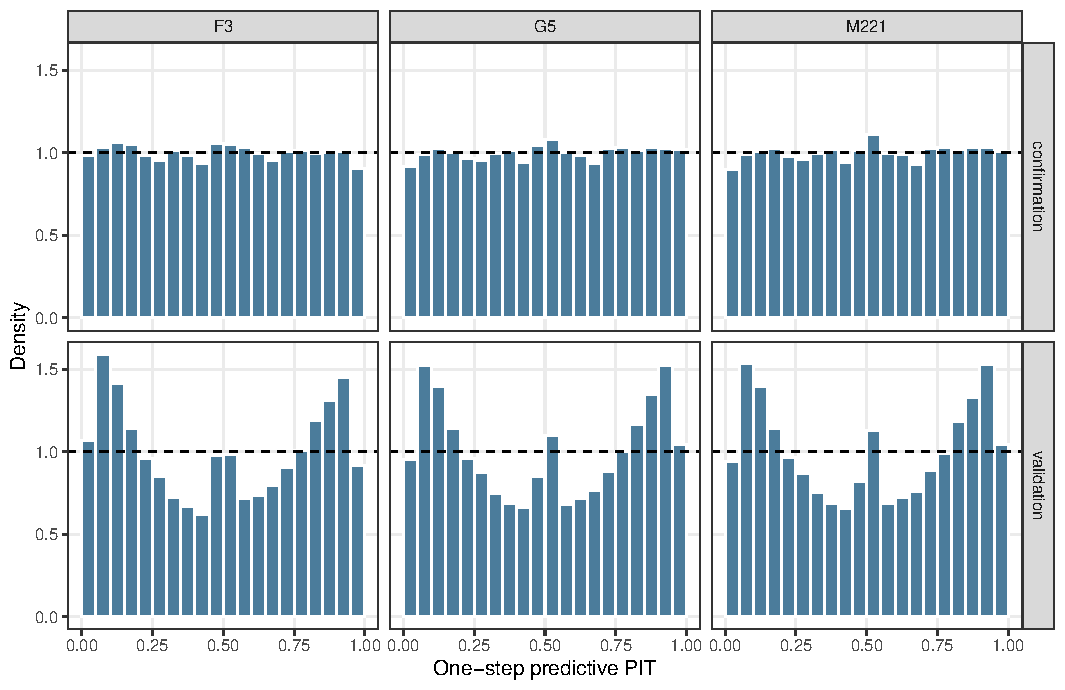
\includegraphics[width=.96\linewidth]{genomic_pit.pdf}
\caption{Predictive PIT values from fixed chromosome-1 estimates. Each row
uses chromosomes excluded from fitting. The dashed line is the uniform
density. The figure shows remaining departures as well as similarities
between the mixture, ordinary and symmetry-aware models.}
\label{fig:si-genomic-pit}
\end{figure}

\subsection{Aggregation, technical replication and sensitivity}

Correspondence between the five G5 states and M221 components minimizes the
sum of squared Hellinger distances between Gaussian emissions. The assignment
uses chromosome-1 emission estimates only; the same map is applied to the
technical replicate and held-out chromosomes. The largest matched distance
is below $10^{-5}$. Aggregated G5 and M221 have 99.73\% agreement on the
estimation markers, 99.07\% on validation and 99.06\% on confirmation. The
unaggregated G5 labels are not interpreted as five distinct regional levels
of allelic imbalance.

Technical replication compares fixed-parameter Viterbi labels at the 19,727
positions shared by the two separately filtered chromosome-1 arrays. M221
agreement is 98.08\%; F3 agreement is 98.04\%. These values measure
repeatability of the fitted assignments on these arrays. They do not estimate
accuracy against independently known states.

\begin{table}[htbp]
\centering
\small
\caption{M221 sensitivity. Agreement is evaluated at markers shared with the primary analysis; parameters are refitted within each scenario.}
\label{tab:si-genomic-sensitivity}
\begin{tabular}{lrrr}
\toprule
Scenario & $n$ & Agreement (\%) & Runs \\
\midrule
$\sigma_{\min}=0.005$ & 20697 & 100.00 & 181 \\
$\sigma_{\min}=0.020$ & 20697 & 100.00 & 181 \\
Every second marker & 10349 & 97.56 & 33 \\
Every fifth marker & 4140 & 96.35 & 20 \\
Normal fraction $[0.25,0.75]$ & 23611 & 98.58 & 302 \\
Normal fraction $[0.35,0.65]$ & 18558 & 98.76 & 55 \\
\bottomrule
\end{tabular}
\end{table}


Sensitivity fits use ten random starts, refinement of the best three for up
to 2,000 iterations, and the primary solution as an additional start. For
thinning by a factor $q$, the warm-start transition matrix is $\Gamma^q$;
parameters are then reestimated. Gaps are evaluated on the retained marker
positions, with the same one-megabase reset rule. Agreement is computed only
at markers present in both versions. Filters can change which marker is kept
at a duplicated position, explaining why the common counts are sometimes
slightly below the smaller sample size. All selected sensitivity fits
converge and have no variance-floor hits. The pronounced reduction in run
counts after thinning is a material limitation for short-segment inference.

The allele-designation experiment uses seed 20260910 to select each
marker independently with probability one half for the transformation $y_i\mapsto1-y_i$, without
refitting. The fixed M221 and G5 log likelihoods change by $-44.23$ and
$-66.54$, respectively. The M221 state path agrees on 99.87\% of markers,
the raw G5 path on 56.63\%, and aggregated G5 on 99.55\%. F2 and F3 are
invariant up to numerical rounding. Approximate invariance of the unconstrained
mixture is an empirical finding, not an imposed property.

\subsection{Genomic comparators and limits of the external reference}

PSCBS 0.68 uses the same candidate heterozygous loci and the total-signal
ratio $2T/N$, with the two chromosome-1 sequences analyzed separately.
We use the default paired segmentation procedure with seeds 20260911 and
20260912. It returns 51 segments. The factor two is the method's relative
copy-number convention; it does not establish absolute tumor ploidy.
PSCBS combines the total signal with allelic imbalance, so it is a
scientific comparator using additional information rather than a fair
BAF-only predictive benchmark. See Olshen et al. (2011),
\url{https://doi.org/10.1093/bioinformatics/btr329}.

The publisher's supplementary sequencing tables for Chiang et al. (2009)
contain 407 HCC1143 segments, extracted with chromosome, start, end, relative
copy ratio and read counts. The original PDF and its hash are recorded;
selected coordinates were checked against the rendered source. The HCC1143
chr1 interval 210,542,048--221,670,720 contains 1,152 retained SNPs. Of these,
1,032 are assigned to the approximately balanced M221 profile, 116 to moderate
imbalance and four to strong imbalance. Published relative copy ratios range
from 1.438 to 2.255 across the interval. In the following published segment,
221,670,740--233,147,476, the relative copy ratio is 1.072, although the allele
fractions are predominantly imbalanced. Total dosage and allelic balance
therefore need separate interpretation.

These sequencing measurements were obtained independently of the arrays, but
they concern the same cell line and measure a different quantity. They cannot
supply true labels for the three HMM profiles. The displayed interval is an
illustration on the development chromosome, selected to explain that
distinction; it is not presented as a reserved validation endpoint. No
clinical claim, absolute copy-number estimate, patient-level performance
claim or novel biological discovery follows from this comparison.


\section{Elk movement: Gaussian comparisons and limitations}\label{sec:elk-si}

Elk movement provides a contrasting case: flexible Gaussian emissions can
improve distributional fit without establishing a behavioral interpretation.
We examine density modes, fitting constraints, temporal prediction and
alternative observation families. The short series and absence of observed
behavior labels limit the interpretation of the fitted states.

\subsection{Input data and matched supplementary measurements}

The analysis reads \texttt{elk\_data} from \texttt{moveHMM} version 1.10 and
checks its structure and serialized SHA-256 digest before fitting. Consecutive
Euclidean displacements are computed separately for each animal, converted
from metres to kilometres and transformed by $\log(1+x)$. The same 735
locations yield 731 within-animal displacements.
Exact observation times are unavailable, so the transition step is a recorded
interval, treated as approximately daily, rather than an exactly measured day.

The original study's supplementary archive
\url{https://doi.org/10.6084/m9.figshare.3523667.v1} provides turning angles,
interval-adjusted daily movement rates and habitat measurements. All 735
animal IDs and coordinate pairs match the package data exactly. The archived
text file also contains 370 empty rows, which are removed before this check.
The file hash, URL and alignment checks are recorded in
\path{empirical/revision2/context_provenance.json}. Auxiliary quantities are
aligned to the departure fix of each outgoing displacement. The first turning
angle of each animal is unavailable. These measurements were not fitted as
responses or used to choose starting values in the Gaussian benchmark.
Section~\ref{sec:movement-si} fits the rates and angles jointly in a separate, support-respecting
analysis.

For elk 163, posterior-weighted mean turning-angle cosines in the M21 states
are $-0.232$ and $-0.261$, respectively. Their mean distances to open forest
are 17.40 and 10.86 km. Neither comparison validates a behavioural label:
angles share the trajectory's measurement errors, while distance to habitat
also changes with the animal's geographic location and does not measure
habitat selection against availability. The full summaries for every fitted
state and animal are in \path{empirical/revision2/context_summary.csv}.
The Gaussian benchmark statement that the regimes differ in displacement
should therefore not be read as a demonstrated contrast in foraging,
travelling or habitat preference.

A targeted check for elk 163 replaces the derived displacements with the
published interval-adjusted rates for the same 158 intervals. With the same
transformation, bound and fitting protocol, the BIC values are 135.1 (G2),
116.0 (G3), 139.8 (G4), 109.1 (M21) and 112.0 (M22). Thus M21 retains a
7.0-point BIC advantage over G3. This check addresses the use of approximate
rather than exact time intervals; it is not an additional independent data
set. Its fitted objects and numerical results are supplied.

\subsection{Estimation, local solutions and boundary checks}

G2, G3 and G4 have 7, 14 and 23 free parameters; M21 and M22 have 10 and 13.
All models estimate an initial distribution and a row-stochastic transition
matrix. The primary bound on component standard deviation is 0.05, with
0.025 and 0.10 used for sensitivity. Each fit starts from 200 seeded random
initializations. After at most 70 screening iterations (relative likelihood
tolerance $10^{-4}$), the best 20 runs are refined at tolerance $10^{-8}$.
Refinement continues in blocks of 2000 iterations, up to 10,000 if needed.
Unrestricted G3 and G4 fits also start at the exact expansion of their M21
and M22 counterparts. Full-series estimates at the three bounds initialize
one another for three additional passes. These warm starts use only the same
full series and are not passed to training-prefix fits.

Every selected fit in the 100-model primary, sensitivity and validation grid
satisfied the stopping rule. All five published-rate fits also converged.
All start-level likelihoods, iteration counts and final increments are
retained. The best refined solution was not always reached by many starts:
for example, the final full-series M21 solution for elk 363 was found by a
cross-bound warm start after the initial screening missed it. This changed
its BIC from 170.8 to 157.4. Reporting convergence alone would miss this
optimization sensitivity. Nested likelihood inequalities and nondecreasing
likelihood as the standard-deviation bound is relaxed are checked explicitly.
These checks do not certify a global optimum.

\begin{table}[tbp]
\centering\small
\caption{Numerical audit at bound 0.05. Gain is the final relative likelihood increment; AtBound counts component standard deviations at the bound. MinTrans and MaxSelf summarize transition boundaries. NearBest counts original refined starts within 0.01 log-likelihood units of the final selected solution, including subsequent warm-start improvements. Convergence of EM does not establish a global maximum.}\label{tab:si-convergence}
\begin{tabular}{llrrrrr}\toprule
Elk & Model & Gain & AtBound & MinTrans & MaxSelf & NearBest \\\midrule
115 & M21 & 5.5e-10 & 0 & 0.0416 & 0.9584 & 1/20 \\
115 & M22 & 2.8e-09 & 1 & 0.0999 & 0.9001 & 20/20 \\
115 & G2 & 2.9e-10 & 0 & 0.1117 & 0.8883 & 20/20 \\
115 & G3 & 3.7e-09 & 1 & 0.0244 & 0.8908 & 20/21 \\
115 & G4 & 4.1e-09 & 1 & 0.0000 & 0.6965 & 20/21 \\
163 & M21 & 6.6e-09 & 1 & 0.2130 & 0.7870 & 20/20 \\
163 & M22 & 4.0e-09 & 2 & 0.2367 & 0.7633 & 20/20 \\
163 & G2 & 3.2e-10 & 0 & 0.2314 & 0.7686 & 20/20 \\
163 & G3 & 5.2e-09 & 1 & 0.1640 & 0.6688 & 21/21 \\
163 & G4 & 3.7e-09 & 2 & 0.0000 & 0.6372 & 17/21 \\
287 & M21 & 3.4e-09 & 0 & 0.1099 & 0.8901 & 20/20 \\
287 & M22 & 9.1e-09 & 0 & 0.0000 & 1.0000 & 20/20 \\
287 & G2 & 2.4e-10 & 0 & 0.1292 & 0.8708 & 20/20 \\
287 & G3 & 2.5e-09 & 0 & 0.0000 & 1.0000 & 21/21 \\
287 & G4 & 7.8e-09 & 0 & 0.0000 & 1.0000 & 20/21 \\
363 & M21 & 7.1e-10 & 0 & 0.0603 & 0.9397 & 0/20 \\
363 & M22 & 1.2e-09 & 0 & 0.0980 & 0.9020 & 4/20 \\
363 & G2 & 4.1e-10 & 0 & 0.3104 & 0.6896 & 19/20 \\
363 & G3 & 8.7e-10 & 0 & 0.0000 & 0.8041 & 20/21 \\
363 & G4 & 9.0e-09 & 1 & 0.0000 & 1.0000 & 19/21 \\
\bottomrule\end{tabular}
\end{table}


The variance-bound counts in Table~\ref{tab:si-convergence} concern emission
standard deviations. Small transition estimates are reported separately;
initial probabilities may also approach the boundary because only one
trajectory is fitted per animal. The near-absorbing M22 state for elk 287 is
particularly consequential for interpreting switching. It is retained as a
limitation, rather than suppressed by an additional transition constraint.

\subsection{Predictive assessment}

For a series of length $T$, the training prefixes end at
$n_1=\lfloor0.6T\rfloor$ and $n_2=\lfloor0.8T\rfloor$. The first fit scores
$n_1+1,\ldots,n_2$, and the second scores $n_2+1,\ldots,T$. Filtering in each
block uses the fitted initial distribution and all preceding observations,
with parameters fixed at their training estimates. No full-series parameter
estimates are used to initialize or score a training-prefix fit. The blocks
are disjoint as scored observations, although the second training set
contains the first validation block. They are consequently not independent
replicates for a significance test.

\begin{table}[tbp]
\centering\small
\caption{Held-out predictive summaries over two disjoint blocks: observations after the first 60\% through 80\%, and after 80\% through the end. Each block uses parameters fitted to its preceding prefix. Coverage is the fraction of PIT values in $[0.05,0.95]$; PIT distance is the empirical Kolmogorov distance. $P(Y<0)$ is the mean predictive probability assigned below the support of the transformed response. Higher log scores are better.}\label{tab:si-predictions}
\begin{tabular}{llrrrrr}\toprule
Elk & Model & $n_{\rm test}$ & Log score & Coverage & PIT distance & $P(Y<0)$ \\\midrule
115 & G2 & 78 & -51.85 & 0.949 & 0.120 & 0.061 \\
115 & G3 & 78 & -47.82 & 0.872 & 0.124 & 0.035 \\
115 & G4 & 78 & -51.34 & 0.936 & 0.081 & 0.039 \\
115 & M21 & 78 & -50.41 & 0.846 & 0.112 & 0.030 \\
115 & M22 & 78 & -51.30 & 0.846 & 0.107 & 0.027 \\
163 & G2 & 64 & -11.49 & 0.984 & 0.172 & 0.081 \\
163 & G3 & 64 & -3.20 & 0.984 & 0.265 & 0.060 \\
163 & G4 & 64 & -9.83 & 0.969 & 0.276 & 0.046 \\
163 & M21 & 64 & 0.02 & 0.969 & 0.172 & 0.048 \\
163 & M22 & 64 & 1.73 & 0.938 & 0.185 & 0.050 \\
287 & G2 & 66 & -52.39 & 1.000 & 0.246 & 0.044 \\
287 & G3 & 66 & -21.03 & 1.000 & 0.173 & 0.040 \\
287 & G4 & 66 & -52.45 & 0.985 & 0.178 & 0.024 \\
287 & M21 & 66 & -42.72 & 1.000 & 0.219 & 0.035 \\
287 & M22 & 66 & -24.33 & 0.985 & 0.228 & 0.019 \\
363 & G2 & 87 & -42.80 & 0.874 & 0.404 & 0.039 \\
363 & G3 & 87 & -28.21 & 0.667 & 0.365 & 0.013 \\
363 & G4 & 87 & -37.12 & 0.632 & 0.383 & 0.010 \\
363 & M21 & 87 & -32.15 & 0.655 & 0.385 & 0.012 \\
363 & M22 & 87 & -35.17 & 0.632 & 0.371 & 0.010 \\
\bottomrule\end{tabular}
\end{table}


The log-score advantage for elk 163 is not uniform across blocks. M21 and G3
score $-7.751$ and $-7.603$ on the first 32 reserved observations, and 7.775
and 4.408 on the final 32. M22 scores $-8.056$ and 9.785. All per-observation
forecasts, PIT values and negative-support probabilities are saved in
\path{empirical/revision2/heldout_predictions.csv}; block totals are in
\path{empirical/revision2/heldout_by_fold.csv}. The retained Gaussian PIT curves and the table use these reserved observations. Full-data density
plots remain descriptive fits and are not predictive validation.

The transformed response is nonnegative, whereas Gaussian approximations
have real-line support. Table~\ref{tab:si-predictions} reports the mean fitted
predictive mass below zero. This mass is not removed by renormalizing the
predictive density after fitting. Accordingly, all model scores refer to the
same real-line observation model, and the support mismatch remains visible
as a limitation.

\subsection{Components, modes and state stability}

\begingroup\small\setstretch{1}
\begin{longtable}{llrrrrrrr}
\caption{Component parameters at bound 0.05. Means and standard deviations are on the transformed scale. Occupation is the average smoothed state probability and Self is the state self-transition probability. Components within a state share the same transition dynamics.}\label{tab:si-parameters}\\
\toprule
Elk & Model & State & Component & Mean & SD & Weight & Occupation & Self \\\midrule\endfirsthead
\toprule
Elk & Model & State & Component & Mean & SD & Weight & Occupation & Self \\\midrule\endhead
115 & M21 & 1 & 1 & 0.458 & 0.243 & 1.000 & 0.517 & 0.958 \\
115 & M21 & 2 & 1 & 0.079 & 0.072 & 0.375 & 0.483 & 0.955 \\
115 & M21 & 2 & 2 & 1.093 & 0.703 & 0.625 & 0.483 & 0.955 \\
115 & M22 & 1 & 1 & 0.057 & 0.050 & 0.202 & 0.835 & 0.900 \\
115 & M22 & 1 & 2 & 0.461 & 0.238 & 0.798 & 0.835 & 0.900 \\
115 & M22 & 2 & 1 & 1.281 & 0.221 & 0.696 & 0.165 & 0.465 \\
115 & M22 & 2 & 2 & 2.341 & 0.223 & 0.304 & 0.165 & 0.465 \\
163 & M21 & 1 & 1 & 0.062 & 0.050 & 0.630 & 0.707 & 0.787 \\
163 & M21 & 1 & 2 & 0.258 & 0.110 & 0.370 & 0.707 & 0.787 \\
163 & M21 & 2 & 1 & 1.486 & 0.784 & 1.000 & 0.293 & 0.469 \\
163 & M22 & 1 & 1 & 0.064 & 0.050 & 0.767 & 0.619 & 0.763 \\
163 & M22 & 1 & 2 & 0.238 & 0.050 & 0.233 & 0.619 & 0.763 \\
163 & M22 & 2 & 1 & 0.460 & 0.209 & 0.446 & 0.381 & 0.603 \\
163 & M22 & 2 & 2 & 1.834 & 0.631 & 0.554 & 0.381 & 0.603 \\
287 & M21 & 1 & 1 & 0.118 & 0.068 & 0.639 & 0.804 & 0.890 \\
287 & M21 & 1 & 2 & 0.432 & 0.173 & 0.361 & 0.804 & 0.890 \\
287 & M21 & 2 & 1 & 1.753 & 0.649 & 1.000 & 0.196 & 0.552 \\
287 & M22 & 1 & 1 & 0.164 & 0.086 & 0.563 & 0.442 & 1.000 \\
287 & M22 & 1 & 2 & 0.466 & 0.135 & 0.437 & 0.442 & 1.000 \\
287 & M22 & 2 & 1 & 0.105 & 0.061 & 0.582 & 0.558 & 0.989 \\
287 & M22 & 2 & 2 & 1.563 & 0.741 & 0.418 & 0.558 & 0.989 \\
363 & M21 & 1 & 1 & 0.459 & 0.238 & 1.000 & 0.317 & 0.857 \\
363 & M21 & 2 & 1 & 0.139 & 0.092 & 0.705 & 0.683 & 0.940 \\
363 & M21 & 2 & 2 & 1.377 & 0.613 & 0.295 & 0.683 & 0.940 \\
363 & M22 & 1 & 1 & 0.345 & 0.171 & 0.753 & 0.495 & 0.892 \\
363 & M22 & 1 & 2 & 0.927 & 0.347 & 0.247 & 0.495 & 0.892 \\
363 & M22 & 2 & 1 & 0.119 & 0.082 & 0.764 & 0.505 & 0.902 \\
363 & M22 & 2 & 2 & 1.692 & 0.510 & 0.236 & 0.505 & 0.902 \\
\bottomrule\end{longtable}

\endgroup

In a mixture-emission HMM, a new component is drawn conditional on the
aggregate state at each observation. Components therefore share the
aggregate transition probabilities and do not carry a separate persistence
parameter. For elk 163, 100\% of G3 state 1 and 87.2\% of G3 state 2 are
assigned to M21 state 1 by the respective Viterbi paths; G3 state 3 maps
entirely to M21 state 2. The assignment is descriptive and does not establish
which partition is biologically correct. The retained M22--G3 comparison
for all animals is shown in Figure~\ref{fig:si-mappings}.

\begin{figure}[tbp]
\centering
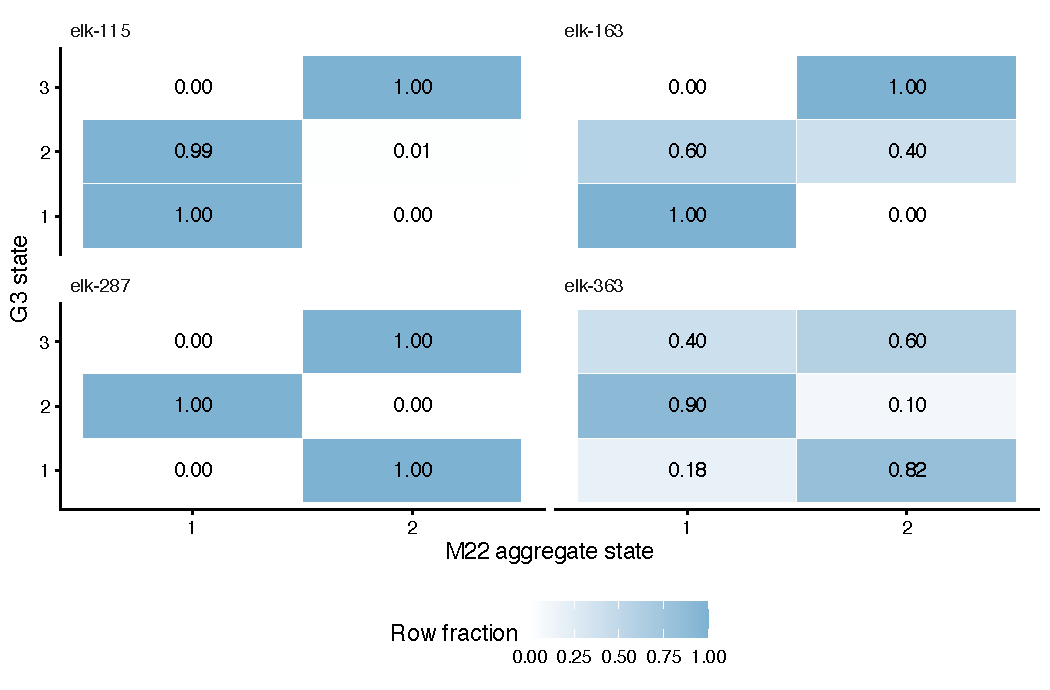
\includegraphics[width=.92\linewidth]{elk_all_mappings.pdf}
\caption{Row proportions mapping full-series G3 Viterbi states to M22 states
for each animal, at standard-deviation bound 0.05, using the refined fits.}
\label{fig:si-mappings}
\end{figure}

\begin{table}[tbp]
\centering\small
\caption{BIC differences across standard-deviation bounds. Negative entries favor the mixture model. The first and third contrasts hold the total number of Gaussian components fixed.}\label{tab:si-sensitivity}
\begin{tabular}{lrrrr}\toprule
Elk & Bound & M21 $-$ G3 & M22 $-$ G3 & M22 $-$ G4 \\\midrule
115 & 0.025 & 11.5 & 13.8 & 4.8 \\
163 & 0.025 & -11.4 & -12.7 & -28.4 \\
287 & 0.025 & 20.5 & -8.7 & -39.2 \\
363 & 0.025 & -8.4 & -8.0 & -9.9 \\
115 & 0.050 & -2.0 & 2.8 & -2.7 \\
163 & 0.050 & -7.8 & -10.8 & -30.2 \\
287 & 0.050 & 20.5 & -8.7 & -39.2 \\
363 & 0.050 & -8.4 & -8.0 & -24.6 \\
115 & 0.100 & -5.4 & 1.4 & -16.3 \\
163 & 0.100 & -7.2 & -5.1 & -33.1 \\
287 & 0.100 & 11.4 & -9.9 & -38.4 \\
363 & 0.100 & -9.9 & -6.3 & -35.3 \\
\bottomrule\end{tabular}
\end{table}


For elk 163, M21--G3 BIC differences remain negative at all three bounds.
After allowing for state-label permutation, the M21 Viterbi paths at bounds
0.025 and 0.10 agree with the primary path on 98.1\% and 93.0\% of intervals.
Thus the broad allocation of low and high displacements is relatively stable,
even though the lower-state density loses a mode at the largest bound.
Mode counts are computed on a 50,001-point grid spanning all fitted
component means plus or minus five standard deviations. Counts describe the
fitted real-line density; they are not estimates of the number of behaviours.

For the four-peak density of elk 115, the component means at bound 0.05 are
0.057, 0.461, 1.281 and 2.341, with standard deviations 0.050, 0.238, 0.221
and 0.223. The density is weighted by posterior state occupation, rather
than assumed stationary occupation. All four peaks can therefore be traced
to specified emission components. Figure~\ref{fig:si-modes} shows the
sensitivity of this shape to the fitting bound. The selected M22 density has
three modes at 0.025 and four at 0.05 and 0.10. The first component is at
the bound in the latter two fits. Neither a four-mode interpretation nor a
claim that only three modes are possible is supported.

\begin{figure}[tbp]
\centering
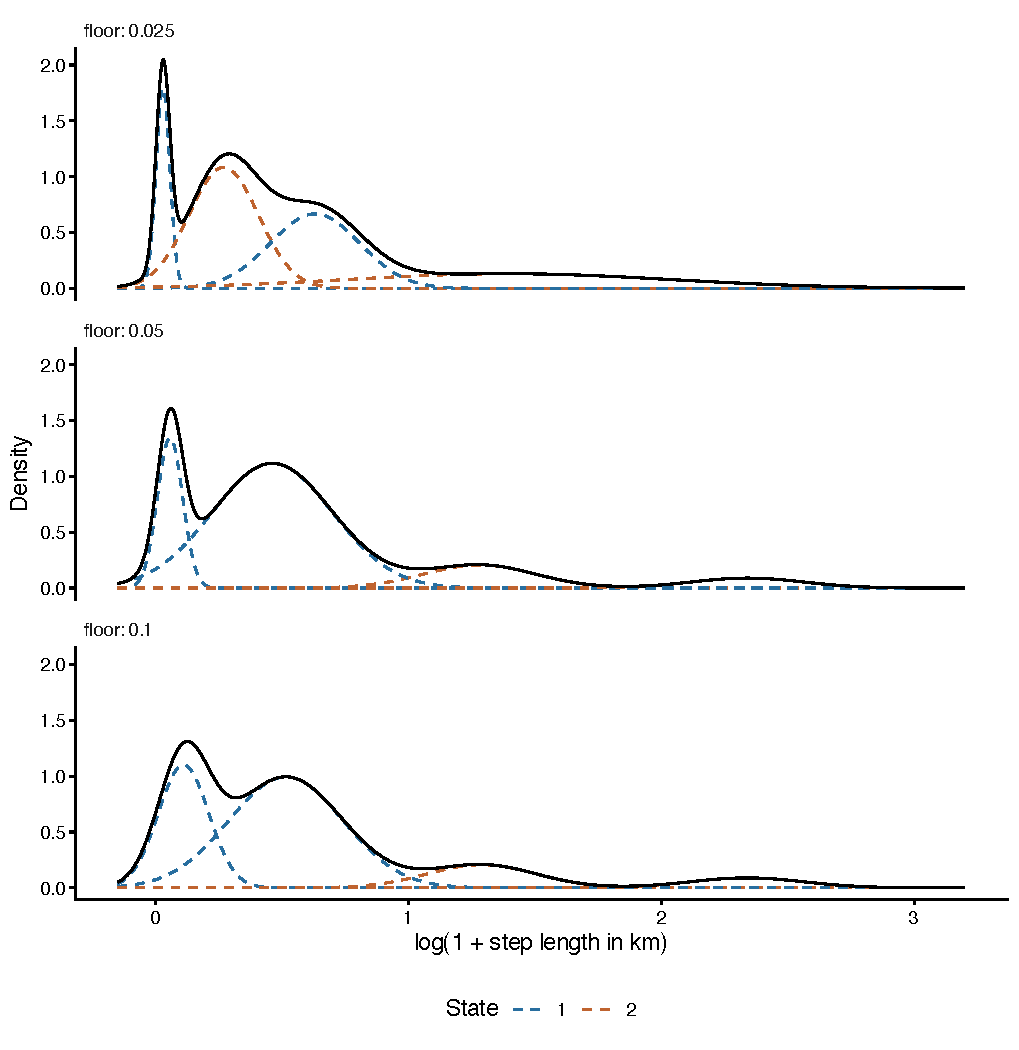
\includegraphics[width=.82\linewidth]{elk115_modes_sensitivity.pdf}
\caption{Elk 115: M22 density decomposition at three standard-deviation
bounds. Dashed curves are the four weighted component contributions, colours
identify aggregate states, and black curves give the total density.}
\label{fig:si-modes}
\end{figure}

\section{Elk movement: joint models and alternative emissions}\label{sec:movement-si}

\subsection{Measurements, observation likelihood and model counts}

The original text archive contains the 735 locations used in the Gaussian
benchmark. Removing its 370 blank rows and matching animal IDs and all
coordinate pairs verifies correspondence with the package data. The new
analysis uses published daily movement rates, which adjust displacement for
the observation interval, rather than reconstructing unavailable timestamps.
Rate and angle refer to the outgoing displacement at a location. The first
angle is unavailable; angles involving the zero-length displacement of
elk 363, or its subsequent displacement, are omitted. There are 731
intervals, one missing rate, 14 reported zero rates and six missing angles
after these omissions. The four animals remain separate likelihoods.

Rates are published to two decimal places. We treat each value as rounded
to the nearest 0.01 km/day. With rate distribution function $F$, the
contribution of value $r$ is
$F(r+0.005)-F(\max(0,r-0.005))$. This observation model avoids assigning
an artificial positive rate to a zero. It is a rounding assumption, not a
model for positional error. Missing response components contribute a
factor of one. The transition recursion continues across their intervals.
Turning angles use a wrapped-Cauchy density with estimated mean direction
and concentration. We condition on an initial state distribution estimated
separately for each trajectory.

The four rate families are gamma (mean and shape), Weibull (scale and shape),
lognormal (log mean and log standard deviation), and a normal distribution
on $\log(1+r)$ truncated below zero. All have two emission parameters per
component. The joint families add two angular parameters per component.
M21 and M22 have component counts $(2,1)$ and $(2,2)$. H2, H3 and H4 have
one component per state. Their rate-only parameter counts are 7, 14, 23,
10 and 13 for H2, H3, H4, M21 and M22; the corresponding joint counts are
11, 20, 31, 16 and 21. BIC uses the number of intervals with at least one
observed response component. It is used descriptively, particularly for
mixtures and near-boundary transition estimates.

\begin{table}[tbp]
\centering\small
\caption{Full-series BIC for rate-only models. Every comparison uses the same rounding intervals and missing-data treatment.}
\label{tab:movement-rate}
\begin{tabular}{llrrrrr}
\toprule
Elk & Family & H2 & H3 & H4 & M21 & M22 \\
\midrule
115 & Gamma & 2190.9 & 2159.8 & 2192.4 & 2167.2 & 2178.3 \\
163 & Gamma & 1682.0 & 1691.0 & 1723.2 & 1683.9 & 1695.0 \\
287 & Gamma & 1742.5 & 1726.0 & 1759.8 & 1715.1 & 1725.5 \\
363 & Gamma & 2350.9 & 2334.3 & 2344.5 & 2318.9 & 2333.9 \\
115 & Weibull & 2180.1 & 2157.0 & 2191.0 & 2168.6 & 2178.1 \\
163 & Weibull & 1680.3 & 1691.1 & 1722.7 & 1684.4 & 1694.4 \\
287 & Weibull & 1744.5 & 1722.7 & 1759.0 & 1712.3 & 1723.8 \\
363 & Weibull & 2351.2 & 2335.1 & 2345.4 & 2319.6 & 2334.6 \\
115 & Lognormal & 2161.4 & 2173.7 & 2197.1 & 2170.5 & 2182.3 \\
163 & Lognormal & 1684.1 & 1696.7 & 1729.7 & 1689.6 & 1700.2 \\
287 & Lognormal & 1747.3 & 1744.1 & 1769.4 & 1732.1 & 1737.3 \\
363 & Lognormal & 2316.8 & 2331.5 & 2349.0 & 2322.7 & 2336.4 \\
115 & Trunc. normal & 2163.6 & 2161.6 & 2191.6 & 2169.9 & 2181.1 \\
163 & Trunc. normal & 1689.6 & 1696.3 & 1726.6 & 1688.6 & 1700.1 \\
287 & Trunc. normal & 1749.4 & 1725.1 & 1760.0 & 1714.7 & 1724.9 \\
363 & Trunc. normal & 2344.7 & 2339.0 & 2347.0 & 2333.6 & 2339.0 \\
\bottomrule
\end{tabular}
\end{table}

\begin{table}[tbp]
\centering\small
\caption{Full-series BIC for joint rate and angle models. Every comparison uses the same rounding intervals and missing-data treatment.}
\label{tab:movement-joint}
\begin{tabular}{llrrrrr}
\toprule
Elk & Family & H2 & H3 & H4 & M21 & M22 \\
\midrule
115 & Gamma & 2891.8 & 2862.2 & 2883.2 & 2865.5 & 2871.9 \\
163 & Gamma & 2256.2 & 2275.6 & 2309.5 & 2264.3 & 2279.8 \\
287 & Gamma & 2319.8 & 2307.8 & 2334.4 & 2296.6 & 2308.8 \\
363 & Gamma & 3129.4 & 3120.4 & 3129.4 & 3107.6 & 3127.2 \\
115 & Weibull & 2881.0 & 2861.0 & 2883.9 & 2866.5 & 2873.3 \\
163 & Weibull & 2254.3 & 2276.1 & 2314.5 & 2264.8 & 2277.9 \\
287 & Weibull & 2319.8 & 2304.2 & 2332.8 & 2293.2 & 2307.1 \\
363 & Weibull & 3129.5 & 3122.2 & 3128.9 & 3109.9 & 3130.0 \\
115 & Lognormal & 2862.4 & 2870.1 & 2885.7 & 2859.6 & 2873.4 \\
163 & Lognormal & 2258.6 & 2281.3 & 2316.3 & 2273.7 & 2278.8 \\
287 & Lognormal & 2326.7 & 2322.1 & 2348.4 & 2312.4 & 2320.4 \\
363 & Lognormal & 3114.7 & 3116.4 & 3141.7 & 3118.1 & 3123.6 \\
115 & Trunc. normal & 2866.1 & 2862.5 & 2886.4 & 2866.0 & 2875.5 \\
163 & Trunc. normal & 2264.6 & 2281.2 & 2316.3 & 2271.1 & 2288.8 \\
287 & Trunc. normal & 2322.2 & 2306.4 & 2335.6 & 2295.3 & 2308.3 \\
363 & Trunc. normal & 3127.3 & 3126.4 & 3134.8 & 3117.2 & 3130.2 \\
\bottomrule
\end{tabular}
\end{table}


The positive-family alternatives change the assessment of elk 163. In
rate-only fits, Weibull H2 has BIC 1680.3, compared with 1684.4 for M21.
In the joint Weibull analysis H2 has BIC 2254.3, below M21 at 2264.8.
The Gaussian mixture result for that animal is therefore sensitive to
emission family. For elk 287, M21 has lower joint BIC than H3 under all
four rate families; this is evidence for a compact fitted representation,
not for identification of the true latent states.

\subsection{Numerical optimization and independent checks}

The binned likelihood is evaluated with log distribution functions and
stable differences in distribution tails. A scaled forward recursion
combines these probabilities with the optional angular densities.
Independent checks compare interval probabilities with R distribution
functions, the forward likelihood with explicit enumeration of short
state sequences, and the two-state mixture with its exact three-state
expansion. Forecast scores telescope to likelihood differences, and changing
a future observation does not change earlier scores. Posterior decoding is
checked against an independently implemented forward--backward recursion.

Full-series fits use 40 random starts, screened for 70 iterations and
180 function evaluations. At least eight are refined for up to 1200
iterations and 3500 evaluations at relative tolerance $10^{-9}$, followed
by a 2000-iteration restart at $10^{-10}$. Selected Weibull and gamma
joint fits use 40 further random starts plus estimates from sensitivity
fits, all re-evaluated on the original full series. The largest improvement
from these additional starts was 8.26 log-likelihood units for gamma M21
on elk 287. This illustrates why an optimizer's stopping code alone does
not establish that competing local solutions were adequately explored.
The final fits, all start-level results and these improvements are retained.

Training-prefix fits initially use 20 starts. The primary Weibull and gamma
joint comparisons receive 80 additional starts each, using only that
prefix's earlier estimates and the nested M21 expansion for H3. Some
training fits also improve materially. No full-series or later-prefix
parameter is supplied as a training start. The full grid contains 160
full-series and 480 training-prefix fits. An optimization audit re-evaluates
every likelihood and computes numerical projected gradients at the bounds.
Optimizer messages and gradient magnitudes are recorded separately;
a successful stopping code is not treated as proof of a global maximum.
Of the 640 selected fits, 639 have a zero optimizer code. One gamma H2
training fit for elk 363 retains a false-convergence message after restarts;
its maximum projected gradient is $3.1\times10^{-5}$. The largest projected
gradient over the grid is 0.00472. The warning remains in the saved results.

Logit parameters are bounded by $\pm12$. The emission ranges are deliberately
broad: positive-family location parameters on a log scale lie in $[-9,5]$;
gamma shape in $[0.05,200]$; Weibull shape in $[0.1,30]$; lognormal and
truncated-normal standard deviations in $[0.05,4]$. The truncated-normal
location lies in $[-3,5]$. Wrapped-Cauchy concentration lies in $[0,0.95]$,
with 0.90 and 0.98 as sensitivity bounds. Numerical boundary estimates are
reported, not interpreted as interior parameter estimates.

\subsection{Five temporal blocks and predictive calibration}

The cutoffs are $\lfloor fT\rfloor$ for $f=0.5,0.6,0.7,0.8,0.9$. Each
fit scores the following tenth of the record, with the final block ending
at $T$. Thus the 97, 79, 82 and 109 scored intervals do not overlap.
Training sets are nested, so block comparisons are dependent. Model families
and the worked case were examined retrospectively; these are not untouched
confirmation sets. Results for every family and animal are retained below.

\begin{table}[tbp]
\centering\small
\caption{Joint predictive log scores over five disjoint blocks. Parameters are estimated on the preceding training prefix only. These retrospective comparisons are exploratory.}
\label{tab:movement-validation}
\begin{tabular}{llrrrr}
\toprule
Elk & Family & H2 & H3 & M21 & M21--H3 \\
\midrule
115 & gamma & -721.4 & -732.5 & -734.2 & -1.7 \\
115 & lognormal & -740.9 & -733.2 & -727.2 & 6.0 \\
115 & Trunc. normal & -736.5 & -726.7 & -728.6 & -1.9 \\
115 & weibull & -721.4 & -735.0 & -738.0 & -3.0 \\
163 & gamma & -520.4 & -524.6 & -525.9 & -1.3 \\
163 & lognormal & -514.2 & -514.6 & -523.0 & -8.3 \\
163 & Trunc. normal & -517.1 & -525.4 & -526.2 & -0.8 \\
163 & weibull & -521.1 & -528.2 & -526.6 & 1.6 \\
287 & gamma & -560.6 & -560.4 & -561.1 & -0.7 \\
287 & lognormal & -558.0 & -554.9 & -553.9 & 1.0 \\
287 & Trunc. normal & -561.9 & -561.9 & -564.6 & -2.7 \\
287 & weibull & -560.9 & -561.0 & -562.2 & -1.3 \\
363 & gamma & -792.8 & -802.1 & -794.5 & 7.6 \\
363 & lognormal & -804.7 & -789.8 & -789.8 & 0.0 \\
363 & Trunc. normal & -784.9 & -788.8 & -788.2 & 0.6 \\
363 & weibull & -791.7 & -796.1 & -785.3 & 10.8 \\
\bottomrule
\end{tabular}
\end{table}


Rate-only and joint log scores concern different response spaces and must
not be compared directly. Rate predictions conditional on past rates and
angles are also saved separately. For binned rates, randomized PIT values
are drawn uniformly between the predictive distribution function at the
lower and upper rounding bounds. One saved randomization is shared across
models for each animal and interval. The central 90\% PIT fraction is a
descriptive calibration check, not an independence test or an interval
estimate for the model's coverage probability.
For elk 287 under Weibull emissions, the within-block lag-one correlations
of normal-score PIT residuals are 0.037 (M21), 0.009 (H3) and 0.062 (H2).
These are descriptive dependence checks without a significance claim.
The central 90\% PIT fraction is 98.8\% for M21 and H2 and 97.6\% for H3,
indicating conservative rate predictions in the scored part of this record.

\begin{figure}[tbp]
\centering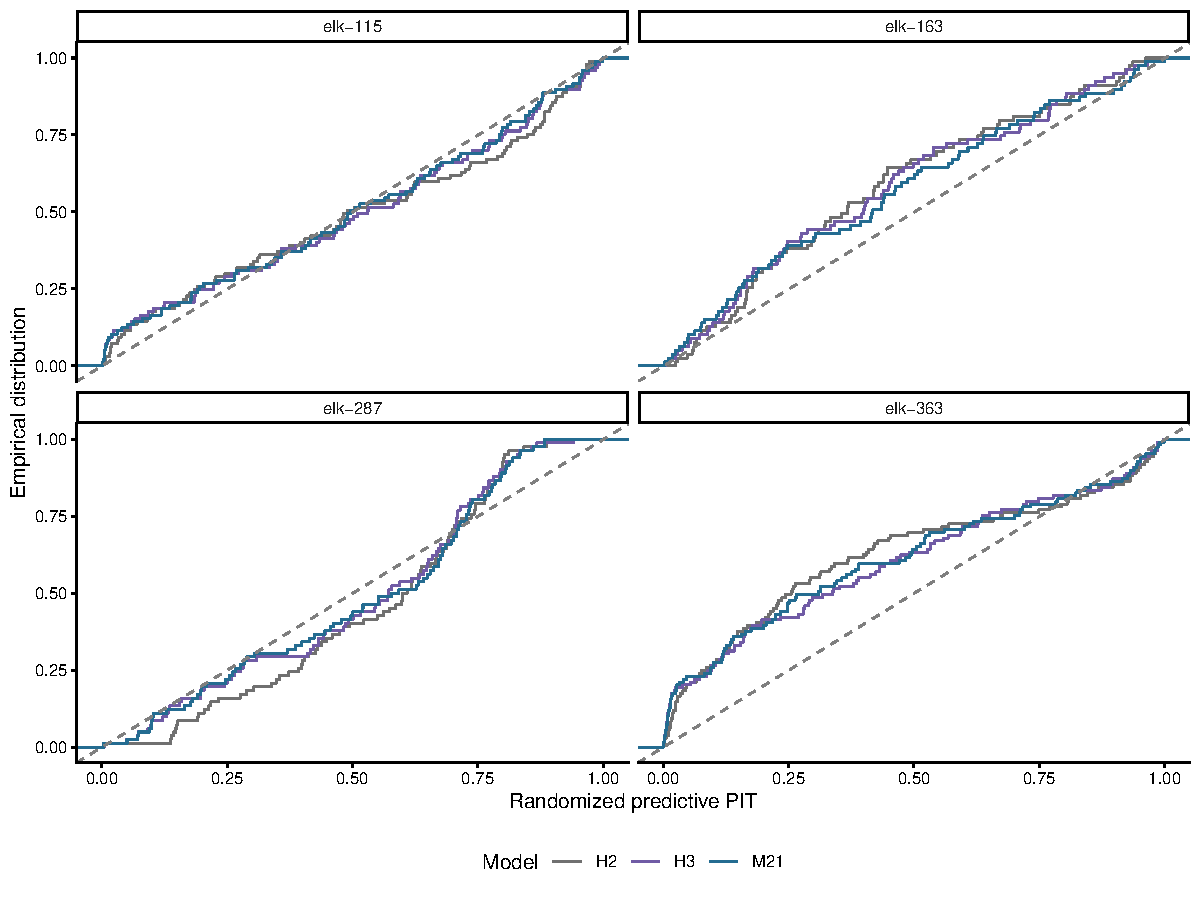
\includegraphics[width=.9\linewidth]{movement_pit.pdf}
\caption{Joint Weibull-model predictive PIT distributions, using the five
scored blocks and a common randomization for rounded rates. The diagonal
is the uniform reference. Deviations remain despite favorable full-data
BIC in some comparisons.}\label{fig:movement-pit}
\end{figure}

The Gaussian benchmark was also extended to the same five cutoffs with
its original 200-start protocol. M21 minus G3 score differences are 1.12,
2.04, $-16.43$ and $-6.22$ for elk 115, 163, 287 and 363, respectively.
The corresponding per-block and per-observation results are retained in
\path{empirical/application_review/gaussian_validation_blocks.csv} and
\path{empirical/application_review/gaussian_validation_predictions.csv}.
Extending the cutoffs does not turn the Gaussian comparison into a uniform
predictive advantage for a mixture.

\subsection{Phase interpretation, resolution and angular heterogeneity}

The joint Weibull M21 fit for elk 287 assigns intervals 1--91 to a mobile
phase and 92--163 to a localized phase. Its two mobile components combine
long directed movements with short, more diffusely oriented movements.
The localized phase's mean rate lies between the means of those components.
It therefore does not represent simply the shortest movements. Maximum
pairwise distances among the locations spanned by each decoded phase are
89.77 and 1.56 km. Median distance to water is 0.460 and 2.071 km. These
are descriptions of the same record, not withheld behavioural measurements.
Raw habitat codes are not interpreted: their correspondence with the
original article's recoded categories is not documented in the data table.

\begin{figure}[tbp]
\centering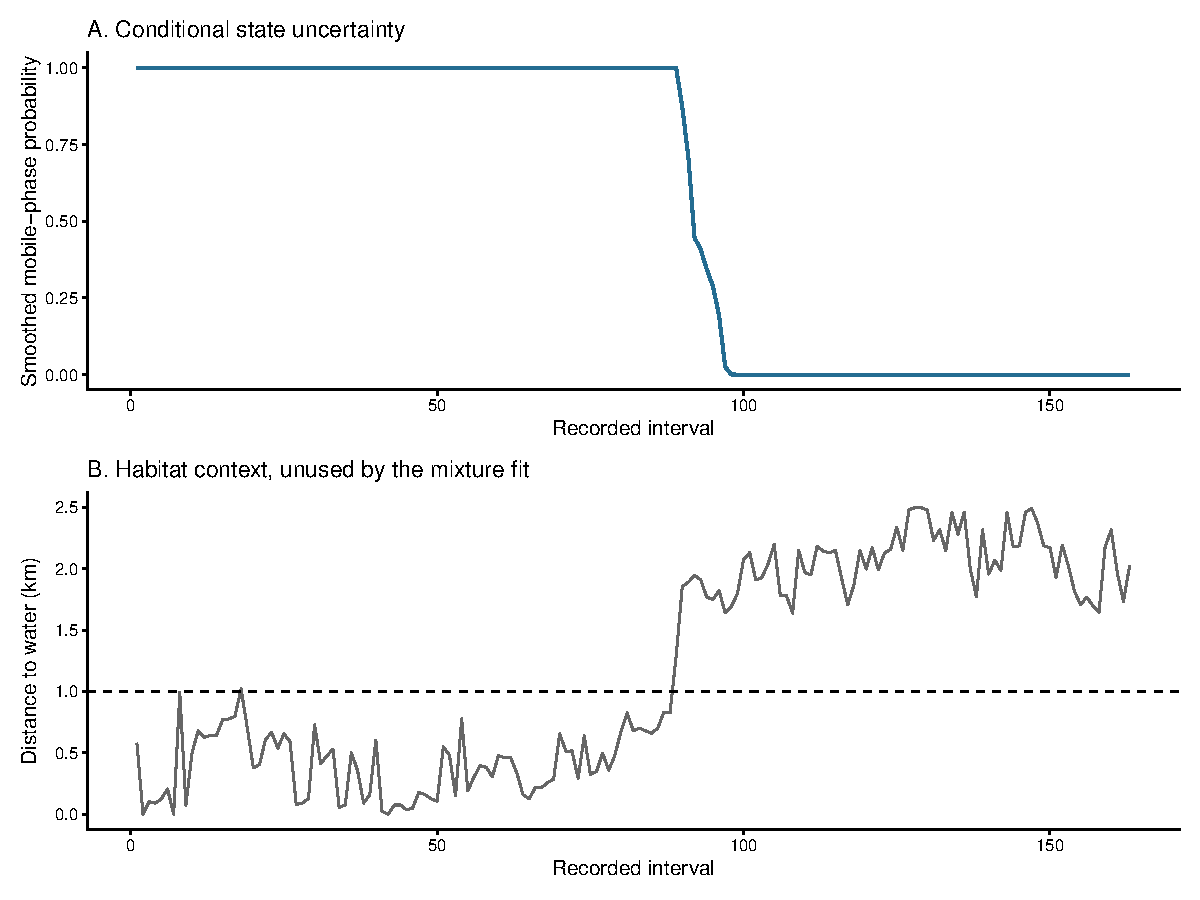
\includegraphics[width=.88\linewidth]{elk_phase_context.pdf}
\caption{Elk 287. Panel A gives the mobile-phase posterior conditional on
the fitted M21 parameters; it does not include parameter uncertainty.
Panel B shows distance to water, which was not fitted by this mixture
model. The dashed line is 1 km and is a descriptive reference, not a
classification threshold.}\label{fig:movement-context}
\end{figure}

To check sensitivity to the smallest movements, values below 0.05 km/day
are grouped into $[0,0.045)$, the union of their original rounding bins.
The analogous grouping below 0.10 is $[0,0.095)$. Angles involving either
small displacement are omitted at each resolution. This changes the
observation being scored, so BIC values are comparable only within the
same coarsening scenario. It does not reproduce a full location-error
likelihood. Both coarsened Weibull M21 fits retain two periods, with 96.9\%
agreement with the original decoding. All other animals are also refitted;
their complete results remain in the reproducibility files.

\begin{table}[tbp]
\centering\small
\caption{Elk 287 sensitivity: BIC comparisons within each row and M21 path agreement with the corresponding uncoarsened family. Coarse 005 and 010 group rates below 0.05 and 0.10 km/day and omit angles involving those small movements. Scores across coarsening scenarios concern different observations and must not be compared.}
\label{tab:movement-sensitivity}
\begin{tabular}{llrrrr}
\toprule
Family & Check & M21 & H2 & H3 & Agreement (\%) \\
\midrule
weibull & coarse 005 & 2183.5 & 2210.8 & 2194.6 & 96.9 \\
gamma & coarse 005 & 2185.3 & 2210.6 & 2196.6 & 96.9 \\
weibull & coarse 010 & 1912.4 & 1930.3 & 1922.9 & 96.9 \\
gamma & coarse 010 & 1914.6 & 1927.1 & 1925.0 & 96.9 \\
weibull & shared angle & 2302.3 & 2319.8 & 2304.2 & 100.0 \\
gamma & shared angle & 2305.1 & 2319.8 & 2307.8 & 98.8 \\
weibull & rho 090 & 2293.2 & 2319.8 & 2304.2 & 100.0 \\
gamma & rho 090 & 2296.6 & 2319.8 & 2307.8 & 100.0 \\
weibull & rho 098 & 2293.2 & 2319.8 & 2304.2 & 100.0 \\
gamma & rho 098 & 2296.6 & 2319.8 & 2307.8 & 100.0 \\
\bottomrule
\end{tabular}
\end{table}


Sharing one angular distribution across both mobile components gives
Weibull M21 14 parameters and BIC 2302.3, compared with 2293.2 for separate
component directions. This comparison suggests that the mixture's role
includes a rate--direction association within the mobile phase. It is not
merely an additional marginal mode. The concentration-bound checks leave
the primary Weibull phase path unchanged.

Only one phase change is observed. The M21 return probability is at the
logit boundary, approximately $6.1\times10^{-6}$. Bounds 8, 12 and 16
give return probabilities approximately $3.4\times10^{-4}$,
$6.1\times10^{-6}$ and $1.1\times10^{-7}$. Their log-likelihoods differ
by about 0.02 and their Viterbi paths are identical. The stable decoding
does not identify an eventual return time or a recurrent ecological
switching process. The near-absorbing interpretation is kept explicit.

\subsection{A competing covariate explanation}

A two-state joint model uses separate logistic regressions for the two
transition rows, with an intercept and slope on the standardized
$\log(1+\text{distance to water in km})$. Standardization uses the training
prefix only. The covariate at the departure location of the current
interval determines its transition probabilities. For validation, these
are conditional forecasts given the current observed location, not
unconditional forecasts of the next location. Zero slopes reproduce the
homogeneous H2 likelihood exactly, which is checked numerically; a short
time-varying example is also checked by enumerating every state sequence.

This model has 13 parameters. For elk 287 the Weibull BIC is 2312.9, an
improvement over homogeneous H2 (2319.8), but above M21 (2293.2). Gamma
gives a similar covariate-model BIC, 2312.8. All four animals and five
training cutoffs are evaluated in
\path{empirical/application_review/water_comparison.csv}. These separate
fits differ from the pooled multi-animal analysis of Patterson et al.
(2017), \url{https://doi.org/10.1007/s10182-017-0302-7}, which motivated
this alternative. One distance covariate cannot exclude other covariates,
explicit phase-change models, time-varying dynamics or measurement error.
No causal water effect, habitat-selection estimate or new species-level
behaviour is inferred.

\section{Reproduction sequence}\label{sec:reproduction}

For the genomic application, run from the reproducibility-package root:
\begin{verbatim}
Rscript genomics/scripts/test_genomic_results.R
Rscript genomics/scripts/test_symmetric_genomic_hmm.R
Rscript genomics/scripts/evaluate_genomic_pilot.R
Rscript genomics/scripts/genomic_diagnostics.R
\end{verbatim}
The supplied processed inputs allow this numerical verification without
reprocessing the microarrays. The genomic README documents a complete
seeded refit and the more demanding route from the four original CEL files,
including exact annotation versions and the R package inventory. It also
records the separate development, validation and confirmation sequence.
Saved fits are evidence for the reported calculations, not substitutes for
these reproduction instructions.

For the retained elk analyses, use the following commands.
Run the following commands from the accompanying reproducibility-package
root, using R and a C++ compiler supported by Rcpp:
\begin{verbatim}
Rscript -e 'renv::restore()'
Rscript numerics/scripts/run_revision_validation.R
Rscript numerics/scripts/refine_revision_sensitivity.R
Rscript numerics/scripts/run_revision_validation.R
Rscript numerics/scripts/check_elk_context.R
Rscript numerics/scripts/render_revision_outputs.R
Rscript numerics/scripts/test_revision.R
\end{verbatim}
The repeated validation command reads the cached fitted objects and refreshes
the summary tables after the cross-bound refinements; it does not refit cached
models. Remove the generated \path{empirical/revision2/fits} directory in a
separate working copy to rerun all estimates from their seeds. The corrected
simulation uses \path{numerics/scripts/run_optimization_audit.R} and
\path{numerics/scripts/refine_reference_simulation.R}, with its protocol
specified in Section S2. The refinement bootstrap is reproduced with
\path{genomics/scripts/genomic_refinement_bootstrap.R}. These scripts retain
checkpointed fits; the package README explains how to rerun them from seeds.

The Gaussian analyses use the existing R EM updates with a compiled version of the
scaled forward--backward recursion. The compiled and R recursions are checked
against one another, and the tests also cover exact refinement, held-out
filtering, likelihood monotonicity, variance-bound sensitivity, normalization,
parameter counts and correspondence between saved fits and numerical tables.
No raw coordinate table is redistributed. Numerical inputs, derived outputs,
model objects, source hashes and session information are documented in
\path{empirical/revision2}.


For the expanded movement analysis, run the following additional sequence.
Cached fits are reused; use a separate copy without the generated
\path{empirical/application_review} directory for a complete seeded rerun.
The input file is downloaded from the archived public source and its
SHA-256 digest is checked before use.
\begin{verbatim}
Rscript numerics/scripts/test_movement_review.R
Rscript numerics/scripts/run_movement_review.R
Rscript numerics/scripts/run_movement_review.R joint
Rscript numerics/scripts/run_movement_validation.R
Rscript numerics/scripts/run_movement_validation.R joint
Rscript numerics/scripts/refine_movement_review.R
Rscript numerics/scripts/run_movement_sensitivity.R
Rscript numerics/scripts/refine_movement_starts.R
Rscript numerics/scripts/refine_movement_validation.R
Rscript numerics/scripts/refine_movement_review.R
Rscript numerics/scripts/run_movement_review.R
Rscript numerics/scripts/run_movement_review.R joint
Rscript numerics/scripts/run_movement_validation.R
Rscript numerics/scripts/run_movement_validation.R joint
Rscript numerics/scripts/run_movement_sensitivity.R
Rscript numerics/scripts/run_water_comparison.R
Rscript numerics/scripts/run_extended_gaussian_validation.R
Rscript numerics/scripts/describe_movement_review.R
Rscript numerics/scripts/check_movement_phase.R
Rscript numerics/scripts/test_movement_results.R
Rscript numerics/scripts/render_movement_review.R
\end{verbatim}

\end{document}
